\section{复合反应}


% \begin{frame}[t]
%     \frametitle{}
%     \begin{question}
%         由于存在多个化学反应，物系中任一反应组分既可能只参与其中一个反应，也可能同时参与其中若干个反应。某一反应既可能是某一反应的反应物，又可能是另一反应的反应产物。在这种情况下，该组分的转化速率该如何表示？
%         \[
%             \ch{A + B ->[k1] C} \qquad r_\mathrm{A1} = k_1c_\mathrm{A}c_\mathrm{B}
%         \]
%         \[
%             \ch{C ->[k2] A + B} \qquad r_\mathrm{A2} = k_2c_\mathrm{C}
%         \]
%     \end{question}
% \end{frame}


\begin{frame}{反应组分的消耗速率或生成速率}
	
    \begin{redblock}{A的转化速率是多少？}
        \[
            \ch{A + B ->[k1] R} \qquad r_\mathrm{A1} = k_1 c_\mathrm{A}c_\mathrm{B}
        \]
        \[
            \ch{A ->[k2] P}  \qquad r_\mathrm{A2} = k_2 c_\mathrm{A}^2
        \]
        \[
            \ch{M + N ->[k3] A} \qquad r_\mathrm{A3} = k_3c_\mathrm{M}c_\mathrm{N}
        \]
    \end{redblock}
	
    复合反应中某组份的反应量是其所参与的各个化学反应共同作用的结果。
	
    我们把单位时间内单位体积反应混合物中某一组份$i$的反应量叫做该组份的\highlight{消耗速率}($i$为反应物)或\highlight{生成速率}($i$为反应产物)，并以符号$\mathcal{R}_i$表示。
\end{frame}




\begin{frame}[t]
    \frametitle{}
    \begin{redblock}{A的转化速率是多少？}
        \[
            \ch{A + B ->[k1] R} \qquad r_\mathrm{A1} = k_1 c_\mathrm{A}c_\mathrm{B}
        \]
        \[
            \ch{A ->[k2] P}  \qquad r_\mathrm{A2} = k_2 c_\mathrm{A}^2
        \]
        \[
            \ch{M + N ->[k3] A} \qquad r_\mathrm{A3} = k_3c_\mathrm{M}c_\mathrm{N}
        \]
        \tcblower
        \[
            \mathcal{R}_\mathrm{A} = r_\mathrm{A3} - r_\mathrm{A1} - r_\mathrm{A2} = k_3c_\mathrm{M}c_\mathrm{N} - k_1 c_\mathrm{A}c_\mathrm{B} - k_2 c_\mathrm{A}^2
        \]
    \end{redblock}
    \begin{itemize}
      \item $\mathcal{R}_i$值若为正，表示该组份在反应过程中是增加的，代表生成速率；
      \item $\mathcal{R}_i$值若为负，表示该组份在反应过程中是减少的，代表消耗速率。
    \end{itemize}
\end{frame}


\begin{frame}[t]
    \frametitle{}
    \begin{question}
        如下反应网络，各物质的净反应速率是？
        \begin{center}
            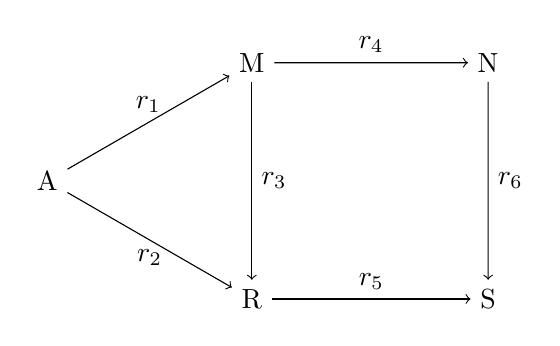
\begin{tikzpicture}[scale=1.5]
                \node (R) at (0,0) {R};
                \node (S) at (2,0) {S};
                \node (M) at (0,2) {M};
                \node (N) at (2,2) {N};
                \node (A) at (150:2) {A};
                \draw [->] (A) -- (M) node [above,midway]{$r_1$};
                \draw [->] (A) -- (R) node [below,midway]{$r_2$};
                \draw [->] (M) -- (N) node [above,midway]{$r_4$};
                \draw [->] (M) -- (R) node [right,midway]{$r_3$};
                \draw [->] (R) -- (S) node [above,midway]{$r_5$};
                \draw [->] (N) -- (S) node [right,midway]{$r_6$};
            \end{tikzpicture}
        \end{center}
    \end{question}
\end{frame}


% \begin{frame}{反应组份的转化速率和生成速率}
% 	$\mathcal{R}_i$应等于按组份$i$计算的各个反应的反应速率的代数和。
% 	$$\mathcal{R}_i=\sum_{j=1}^{M} \nu_{ij}\overline{r}_j$$
% 	\\$\overline{r}_j$为第$j$个反应式的反应速率，乘以组份$i$在第$j$个反应中的化学计量系数$\nu_{ij}$，则得按组份$i$计算的第$j$个反应的反应速率。
% 	\begin{itemize}
%       \item $\mathcal{R}_i$值若为正，表示该组份在反应过程中是增加的，代表生成速率；
%       \item $\mathcal{R}_i$值若为负，则情况相反，代表消耗速率，或转化速率。
%     \end{itemize}
	
%     $\mathcal{R}_i$与反应速率$r_i$的区别在于前者是针对若干反应，而后者则是对一个反应而言。如果只进行一个反应，$r_i=|\mathcal{R}_i|$
% \end{frame}



% \begin{frame}[t]
%     \frametitle{}
%     \begin{example}
%         对于可逆反应
%         \[
%             \ch{A + B <=>[k1][k2] C}
%         \]
%         实质上由两个反应所组成：
%         \[
%             \ch{A + B ->[k1] C} \qquad r_\mathrm{A1} = k_1c_\mathrm{A}c_\mathrm{B}
%         \]
%         \[
%             \ch{C ->[k2] A + B} \qquad r_\mathrm{A2} = k_2c_\mathrm{C}
%         \]
%         则反应组分A的净反应速率为：
%         \[
%             \mathcal{R}_\mathrm{A} = r_\mathrm{A2} - r_\mathrm{A1} = k_2c_\mathrm{C} - k_1c_\mathrm{A}c_\mathrm{B}
%         \]
%     \end{example}
% \end{frame}


\begin{frame}[t]
    \frametitle{}
    \vspace{-5pt}
    \begin{block}{例2.4}
        高温下将乙烷进行热裂解以生产乙烯，其反应及速率方程如下：
		$$\begin{array}{r}
		\ce{C2H6 <=> C2H4 + H2}\\
		\ce{2C2H6 -> C3H8 + CH4}\\
		\ce{C3H6 <=> C2H2 + CH4}\\
		\ce{C2H2 + C2H4 -> C4H6}\\
		\ce{C2H4 + C2H6 -> C3H6 + CH4}
	\end{array}~~~~~~~~~~~~
	\begin{array}{l}
		\overline{r}_1=\overrightarrow{k}_1c_\mathrm{A}-\overleftarrow{k}_1c_\mathrm{E}c_\mathrm{H}\\
		\overline{r}_2=\overrightarrow{k}_2c_\mathrm{A}\\
		\overline{r}_3=\overrightarrow{k}_3c_\mathrm{P}-\overleftarrow{k}_3c_\mathrm{R}c_\mathrm{M}\\
		\overline{r}_4=\overrightarrow{k}_4c_\mathrm{R}c_\mathrm{E}\\
		\overline{r}_5=\overrightarrow{k}_5c_\mathrm{E}c_\mathrm{A}
	\end{array}$$
    式中，下标A，R，E，P，M和H分别代表\ce{C2H6}、 \ce{C2H2}、 \ce{C2H4}、 \ce{C3H6}、 \ce{CH4}和 \ce{H2}。试导出乙烷的转化速率，乙烯的生成速率表达式。
    \tcblower
    \pause
        \[
            \mathcal{R}_\mathrm{A} = -r_\mathrm{1} - 2r_\mathrm{2} - r_\mathrm{5} = -\overrightarrow{k}_1c_\mathrm{A} + \overleftarrow{k}_1c_\mathrm{E}c_\mathrm{H} - 2\overrightarrow{k}_2c_\mathrm{A} - \overrightarrow{k}_5c_\mathrm{E}c_\mathrm{A}
        \]
        \[
            \mathcal{R}_\mathrm{E} = r_\mathrm{1} - r_\mathrm{4} - r_\mathrm{5} = \overrightarrow{k}_1c_\mathrm{A}-\overleftarrow{k}_1c_\mathrm{E}c_\mathrm{H} - \overrightarrow{k}_4c_\mathrm{R}c_\mathrm{E} - \overrightarrow{k}_5c_\mathrm{E}c_\mathrm{A}
        \]
    \end{block}
\end{frame}


\begin{frame}[t]
    \frametitle{}
    \begin{redblock}{习题2.9}
        在一恒容反应器中进行下列液相反应 ：
        \[
            \ch{A + B -> R} \qquad r_\mathrm{R} = 1.6 c_\mathrm{A}
        \]
        \[
            \ch{2 A -> D}  \qquad r_\mathrm{D} = 8.2 c_\mathrm{A}^2
        \]
        式中$r_\mathrm{R}$、$r_\mathrm{D}$分别表示产物 R 及 D 的生成速率，其单位均为 \si{kmol.m^{-3}.h^{-1}}， 反应用的原料为 A 与 B 的混合物 ， 其中 A 的浓度为 \SI{2}{kmol.m^{-3}} ， 试计算 A 的转化率达 95\%时所需要的反应时间 。
        \tcblower
        \pause
        \[
            \mathcal{R}_\mathrm{A} = -r_\mathrm{R} - 2r_\mathrm{D} = -1.6 c_\mathrm{A} - 16.4c_\mathrm{A}^2
        \]
        \[
            -\frac{\dif c_\mathrm{A}}{\dif t} = -\mathcal{R}_\mathrm{A} = 1.6 c_\mathrm{A} + 16.4 c_\mathrm{A}^2
        \]
    \end{redblock}
\end{frame}


\begin{frame}[t]
    \frametitle{}
    \vspace{-5pt}
    \begin{block}{例2.4 改}
		$$\begin{array}{r}
		\ce{C2H6 <=> C2H4 + H2}\\
		\ce{2C2H6 -> C3H8 + CH4}\\
		\ce{C3H6 <=> C2H2 + CH4}\\
		\ce{C2H2 + C2H4 -> C4H6}\\
		\ce{C2H4 + C2H6 -> C3H6 + CH4}
	\end{array}~~~~~~~~~~~~
	\begin{array}{l}
		r_1=?\\
		r_2=?\\
		r_3=?\\
		r_4=?\\
		r_5=?
	\end{array}$$
    通过实验测得\ce{C2H6}、 \ce{C2H2}、 \ce{C2H4}、 \ce{C3H6}、 \ce{CH4}和 \ce{H2}的消耗速率或生成速率$\mathcal{R}_\mathrm{A}$，$\mathcal{R}_\mathrm{R}$，$\mathcal{R}_\mathrm{E}$，$\mathcal{R}_\mathrm{P}$，$\mathcal{R}_\mathrm{M}$，$\mathcal{R}_\mathrm{H}$，如何求各反应的反应速率？
    \tcblower
    \pause
        \[
            \mathcal{R}_\mathrm{A} = -r_\mathrm{1} - 2r_\mathrm{2} - r_\mathrm{5}
        \]
        \[
            \mathcal{R}_\mathrm{E} = r_\mathrm{1} - r_\mathrm{4} - r_\mathrm{5}
        \]
    \end{block}
\end{frame}


\begin{frame}{如何得到复合反应中各反应的反应速率？}
	复合反应动力学实验测量得到的是各个反应综合的结果，即反应组分的生成速率或消耗速率。动力学研究最关心的是各个反应的反应速率，因之就存在一个如何由$\mathcal{R}_i$求$\overline{r}_j$的问题。
	\begin{itemize}
		\item 明确系统中有哪些反应，并分清主次。
		\item 忽略次要反应，只考虑起主要作用的反应。
		\item 设所要考虑的反应数目为M，通过实验测定不少于M个组分的生成速率或消耗速率。
		\item 得到M个线性代数方程，解之得各个反应的反应速率$\overline{r}_j$。
	\end{itemize}
	~~~~~~~~应注意，这M个反应必须是独立反应。所谓独立反应是指这些反应中任何一个反应都不可能由其余反应进行线性组合而得到。
\end{frame}


\begin{frame}{独立反应数的确定}
	以甲烷水蒸汽转化反应为例：
    \[
        \ch{CH4 + H2O <=> CO + 3 H2} \qquad \quad (1)
    \]
    \[
        \ch{CH4 + 2 H2O <=> CO2 + 4 H2} \qquad (2)
    \]
    \[
        \ch{CO + H2O <=> CO2 + H2} \qquad \quad \quad (3)
    \]
	其中只有两个是独立反应，因为其中总有一个反应可由其余两个线性组合得到，

    例如$(1)+(3)=(2)$
\end{frame}


\begin{frame}[fragile]
    \frametitle{通过化学计量系数矩阵得到独立反应数}
	对于化学计量系数矩阵A，其元素由全部5个反应组分在对应的3个化学反应式中的化学计量系数构成。
	$$\mathrm{CH_4~H_2~H_2O~CO~CO_2}$$
	$$\mathrm{A} = \begin{pmatrix}
	-1&  3&  -1&  -1& 0\\
	-1&  4&  -2&  0& 1\\
	0&  1&  -1&  -1& 1
\end{pmatrix}~~~~
\begin{matrix}
	(1)\\
	(2)\\
	(3)
\end{matrix}$$
	\\经初等变换后，求得矩阵A的秩$R(\mathrm{A})=2$，此时独立反应数等于矩阵的秩。
    \begin{codeblock}{使用Matlab计算矩阵A的秩}
A = [-1 3 -1 1 0; -1 4 -2 0 1; 0 1 -1 -1 1];
rank(A) # 返回结果 2
    \end{codeblock}
\end{frame}


\begin{frame}{通过原子系数矩阵得到独立反应数}
	在未知化学反应式的情况下，还可根据反应组分确定独立反应数。将反应式中所包含的全部元素种类，按分别出现在5个反应组分中的原子个数，写成原子系数矩阵B。
	$$\mathrm{CH_4~H_2~H_2O~CO~CO_2}$$
	$$\mathrm{B} = \begin{pmatrix}
		1&  0&  0&  1& 1\\
		4&  2&  2&  0& 0\\
		0&  0&  1&  1& 2
	\end{pmatrix}~~~~~~ 
	\begin{matrix}
		\mathrm{C}\\
		\mathrm{H}\\
		\mathrm{O}
	\end{matrix}$$
	\\求得矩B的秩$R(\mathrm{B})=3$，此时的独立反应数等于反应组分数$-R(\mathrm{B})$
	$$5-3=2$$
	\end{frame}


\begin{frame}{复合反应的基本类型}
	复合反应包括三个基本类型：
	\begin{itemize}
		\item 并列反应\par 反应系统中各个反应的反应组分各不相同
		\item 平行反应\par 反应物完全相同而反应产物不相同或不全相同
		\item 连串反应\par 一个反应的反应产物同时又是另一个反应的反应物
	\end{itemize}
	可逆反应亦属复合反应之列，但它可按单一反应的办法来处理，所以不将它包括在内。
\end{frame}


\begin{frame}{并列反应}
    \[
        \ch{A -> P}
    \]
    \[
        \ch{B -> Q}
    \]
	各个反应都可按单一反应来处理而得到相应的速率方程。
	
    任一个反应的反应速率不受其他反应的反应组分浓度的影响，因此，各个反应独立进行是并列反应的动力学特点。
    \begin{alertblock}
        例外情况：
        \begin{enumerate}
          \item 某些多相催化反应
          \item 变容反应
        \end{enumerate}
    \end{alertblock}
\end{frame}


\begin{frame}{平行反应}
    \[
        \ch{A -> P} \qquad r_\mathrm{P}=k_1c_\mathrm{A}^\alpha
    \]
    \[
        \ch{$\nu_\mathrm{A}$ A ->Q} \qquad r_\mathrm{Q}=k_2c_\mathrm{A}^\beta
    \]
	如果我们的目的是生产P，则P称为\highlight{目的产物}(或主产物)，其它产物均称\highlight{副产物}。
	
	生成主产物的反应称\highlight{主反应}，其它的均称为\highlight{副反应}。
	
    研究复合反应的目标之一是加快主反应的速率，降低副反应的速率，以获得尽可能多的目的产物。通常用\highlight{瞬时选择性}来评价主副反应速率相对大小。
    \[
        S=\mu_\mathrm{PA}\frac{\mathscr{R}_\mathrm{P}}{|\mathscr{R}_\mathrm{A}|}=\mu_\mathrm{PA}\frac{\mbox{目的产物的生成速率}}{|\mbox{关键反应物的消耗速率}|}
    \]
	式中，$\mu_\mathrm{PA}$为生成1molP所消耗的A的mol数。用瞬时选择性这个词，是要表明其值随反应物系的组成及温度而变，它是一个瞬时值。
\end{frame}


\begin{frame}{浓度对平行反应瞬时选择性的影响}
	\[
        S=\frac{k_1c_\mathrm{A}^\alpha}{k_1c_\mathrm{A}^\alpha+|{\nu_\mathrm{A}}|k_2c_\mathrm{A}^\beta}=\frac{1}{1+\frac{k_2}{k_1}|{\nu_\mathrm{A}}|c_\mathrm{A}^{\beta -\alpha}}
    \]
	若温度一定，则$k_1$和$k_2$为常数，反应物浓度$c_\mathrm{A}$改变时，瞬时选择性的变化与主副反应级数有关。
    \only<1>{
    \begin{itemize}
		\item  当$\alpha = \beta$时，S与浓度无关，仅为温度的函数
		\item  当$\alpha > \beta$时，反应物浓度提高，S会？？？
		\item  当$\alpha < \beta$时，反应物浓度提高，S会？？？
	\end{itemize}    
    }
    \only<2>{
    \begin{itemize}
		\item  当$\alpha = \beta$时，S与浓度无关，仅为温度的函数
		\item  当$\alpha > \beta$时，反应物浓度提高，S增加，高浓度操作有利
		\item  当$\alpha < \beta$时，反应物浓度提高，S减小，低浓度操作有利
	\end{itemize}
    }
\end{frame}


\begin{frame}{温度对平行反应瞬时选择性的影响}
	设主副反应的活化能分别为$E_1$和$E_2$，且反应速率常数$k_1$和$k_2$与温度的关系符合阿伦尼乌斯公式，则
    \[
        S=\frac{1}{1+\frac{A_2}{A_1}\exp(\frac{E_1-E_2}{RT})|{\nu_\mathrm{A}}|c_\mathrm{A}^{\beta -\alpha}}
    \]
	当浓度一定时，温度对瞬时选择性的影响取决于主副反应活化能的相对大小。
    
    \begin{itemize}
		\item 当$E_1> E_2$时，温度越高，反应的瞬时选择性越大
		\item 当$E_2> E_1$时，温度升高，反应的瞬时选择性降低
	\end{itemize}
	
\end{frame}


\begin{frame}{连串反应}
    \[
        \ch{A ->[k1] P ->[k2] Q} \qquad r_\mathrm{P} = k_1c_\mathrm{A}^\alpha - k_2c_\mathrm{P}^\beta
    \]
    \begin{itemize}
      \item 无论目的产物是P还是Q，提高反应物A的转化率总是有利的
      \item Q为目的产物时，加速这两个反应都是有利的。可采用高温高浓度的方法。
      \item 若目的产物为P，则应使第二个反应的速率尽可能的慢，以获得更多的产品P。
      \item 由于P能进一步转化成Q，因此，中间产物P必然存在一最大收率，反应进行应适可而止，不能过度。
      \item 选择有利于第一个反应而抑制第二个反应的催化剂，是提高P收率的有效方法。
    \end{itemize}
\end{frame}


\begin{frame}[t]
    \frametitle{}
    \begin{block}{例2.4}
        高温下将乙烷进行热裂解以生产乙烯，其反应及速率方程如下：
		$$\begin{array}{r}
		\ce{C2H6 <=> C2H4 + H2}\\
		\ce{2C2H6 -> C3H8 + CH4}\\
		\ce{C3H6 <=> C2H2 + CH4}\\
		\ce{C2H2 + C2H4 -> C4H6}\\
		\ce{C2H4 + C2H6 -> C3H6 + CH4}
	\end{array}~~~~~~~~~~~~
	\begin{array}{l}
		\overline{r}_1=\overrightarrow{k}_1c_\mathrm{A}-\overleftarrow{k}_1c_\mathrm{E}c_\mathrm{H}\\
		\overline{r}_2=\overrightarrow{k}_2c_\mathrm{A}\\
		\overline{r}_3=\overrightarrow{k}_3c_\mathrm{P}-\overleftarrow{k}_3c_\mathrm{R}c_\mathrm{M}\\
		\overline{r}_4=\overrightarrow{k}_4c_\mathrm{R}c_\mathrm{E}\\
		\overline{r}_5=\overrightarrow{k}_5c_\mathrm{E}c_\mathrm{A}
	\end{array}$$
    式中，下标A，R，E，P，M和H分别代表\ce{C2H6}、 \ce{C2H2}、 \ce{C2H4}、 \ce{C3H6}、 \ce{CH4}和 \ce{H2}。试导出生成乙烯的瞬时选择性表达式。
    \end{block}
\end{frame}


\begin{frame}{反应网络}
	前面介绍的复合反应的三种基本类型，各有各自的特点，实际反应系统同时兼有这三种类型的也不少见，这样复杂的反应系统，往往构成一个网络，称之为反应网络。
	\begin{columns}[c]
	\column{7cm}
	\begin{center}
		\begin{tikzpicture}[scale=1.5]
			\node (C) at (0,0) {C};
			\node (D) at (2,0) {D};
			\node (B) at (0,2) {B};
			\node (A) at (150:2) {A};
			\draw [->] (A) -- (B) node [above,midway]{1};
			\draw [->] (A) -- (C) node [above,midway]{2};
			\draw [->] (B) -- (C) node [right,midway]{3};
			\draw [->] (C) -- (D) node [above,midway]{4};
		\end{tikzpicture}
	\end{center}
	
	\column{7cm}
	\begin{itemize}
		\item 反应1，2构成平行反应
		\item 反应1，3，4构成连串反应
		\item 反应2，4构成连串反应
	\end{itemize}	
		\end{columns}
		\bigskip

		随着反应数目的增多，反应系统的动力学表征将变得越来越复杂，解决办法是将反应网络简化。
	
\end{frame}